% для компиляции в lualatex!!
\documentclass[12pt, a4paper]{article}
\usepackage[english,russian]{babel}
\usepackage[warn]{mathtext}
%\usepackage[T2A]{fontenc}
%\usepackage[utf8]{inputenc}

\usepackage{xecyr} % Продукт Вашего покорного слуги ;)

\setmainfont{DejaVu Serif}

\usepackage{color}
\usepackage{amssymb,amsmath}
\usepackage{graphicx}
\usepackage{multicol}

\textheight=24cm           % высота текста
\textwidth=16cm            % ширина текста
\oddsidemargin=0pt         % отступ от левого края
\topmargin=-1.5cm          % отступ от верхнего края
\parindent=24pt            % абзацный отступ
\parskip=0pt               % интервал между абзацами
\tolerance=2000            % терпимость к "жидким" строкам
\flushbottom               % выравнивание высоты страниц
%\def\baselinestretch{1.5} % печать с большим интервалом

\title{Динамика литоральных поселений {\it Macoma balthica} в вершине Кандалакшского залива Белого моря.}
\author{С.~А.~Назарова \thanks{e-mail:~sophia.nazarova@gmail.com}, Д.~А.~Аристов, А.~В.~Полоскин}
%\date{}

\begin{document}

\maketitle

\section{Введение}

\section{Материал и методика}
Материал для данной работы был собран в ходе экспедиций Группы исследований прибрежных сообществ Лаборатории экологии морского бентоса (гидробиологии) СПбГДТЮ в акватории Кандалакшского государсвтенного заповедника и граничащей с ним зоне. 
Мониторинг плотных поселений {\it Macoma balthica} проводили на 6 участках литорали (рис. \ref{ris:map_Kandalaksha}).
Сборы проводили с 1992 по 2012 год ежегодно в период с 15 июля по 10 августа.\textcolor{red}{какие реально даты?}

Структура материала представлена в таблице \ref{tab: material_Kandalaksha}.
\begin{table}
\begin{tabular}{|*{5}{p{0.2\textwidth}|}} \hline
участок & годы наблюдения & обследованные горизонты литорали & количество проб в однократной съемке & площадь пробоотборника  \\ \hline
о. Горелый Лувеньгских шхер & 1992 -- 2012 & & & \\ \hline
Материковая литораль в районе пос. Лувеньга & 1992-2000, 2002, 2004 & & & \\ \hline
Эстуарий р. Лувеньги & 1992 -- 2012 & & & \\ \hline
Литораль Западной Ряшковой салмы о. Ряшкова & 1994 -- 2012 & & & \\ \hline
Южная губа о. Ряшкова & 2001 -- 2012 & & & \\ \hline
о. Ломнишный & 2007 -- 2012 & & &  \\ \hline
\end{tabular}
\caption{Структура использованного в работе материала}
\label{tab:material_Kandalaksha}
\end{table}

На каждом исследованном участке отбирали 3 --- 20 проб площадью 1/30 --- 1/10 м^2, котрые затем промывали на сите с диаметром ячеи 1 мм.

\subsection{Динамика обилия {\it M.~balthica}}
\subsubsection{Эстуарий р.~Лувеньги.}



%Эстуарий Лувеньги


\begin{figure}[h]

\begin{multicols}{3}
\hfill
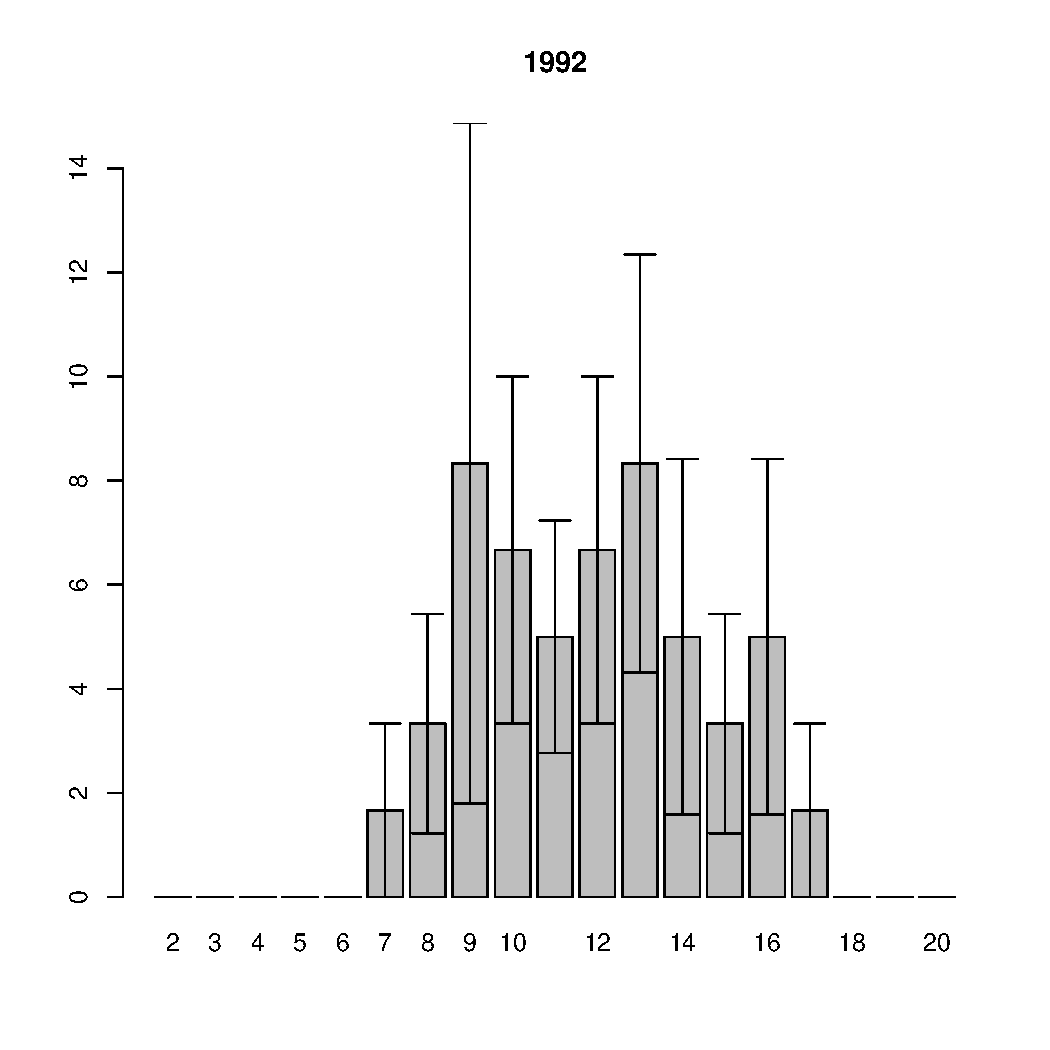
\includegraphics[width=65mm]{../White_Sea/Estuatiy_Luvenga/sizestr2_1992_.pdf}
\hfill
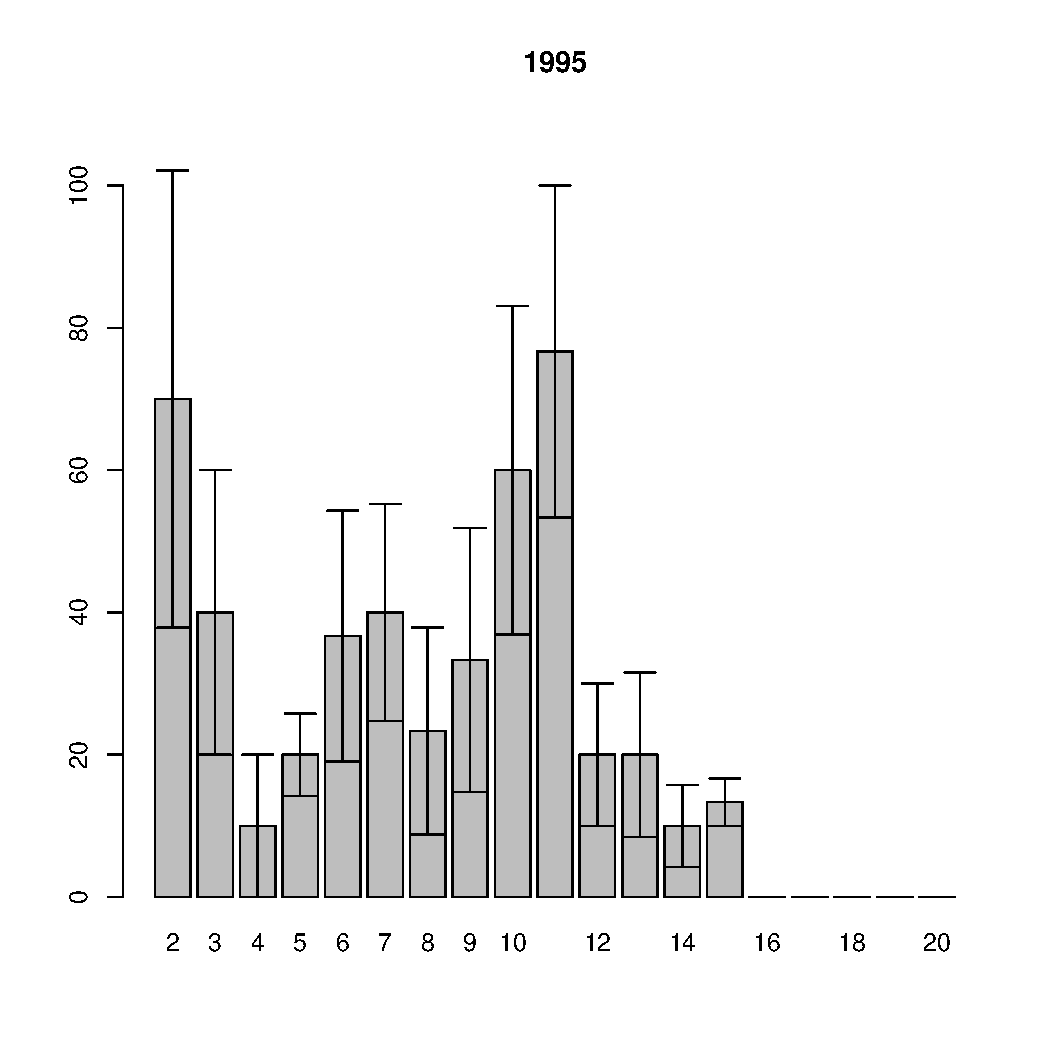
\includegraphics[width=65mm]{../White_Sea/Estuatiy_Luvenga/sizestr2_1995_.pdf}

\hfill
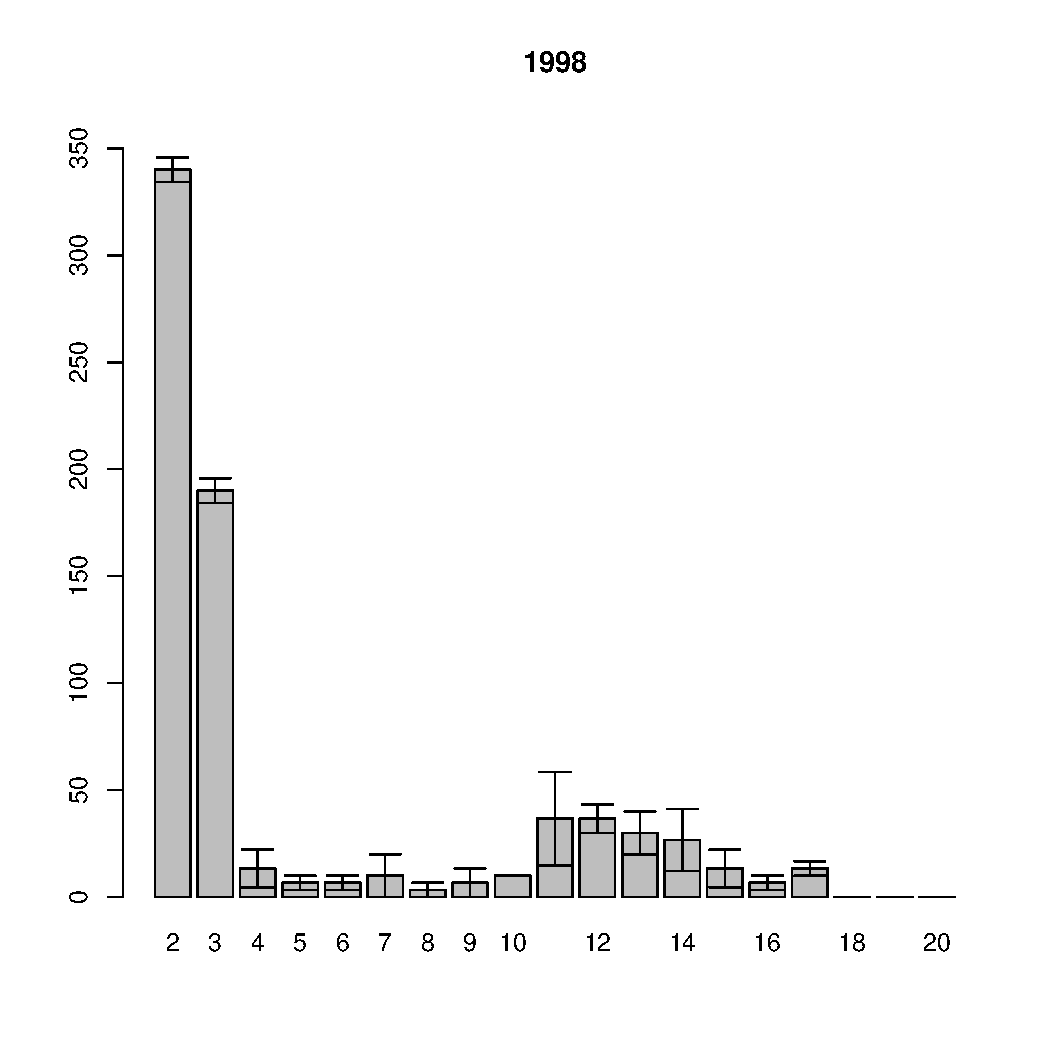
\includegraphics[width=65mm]{../White_Sea/Estuatiy_Luvenga/sizestr2_1998_.pdf}

\end{multicols}

%\smallskip


\begin{multicols}{3}
\hfill
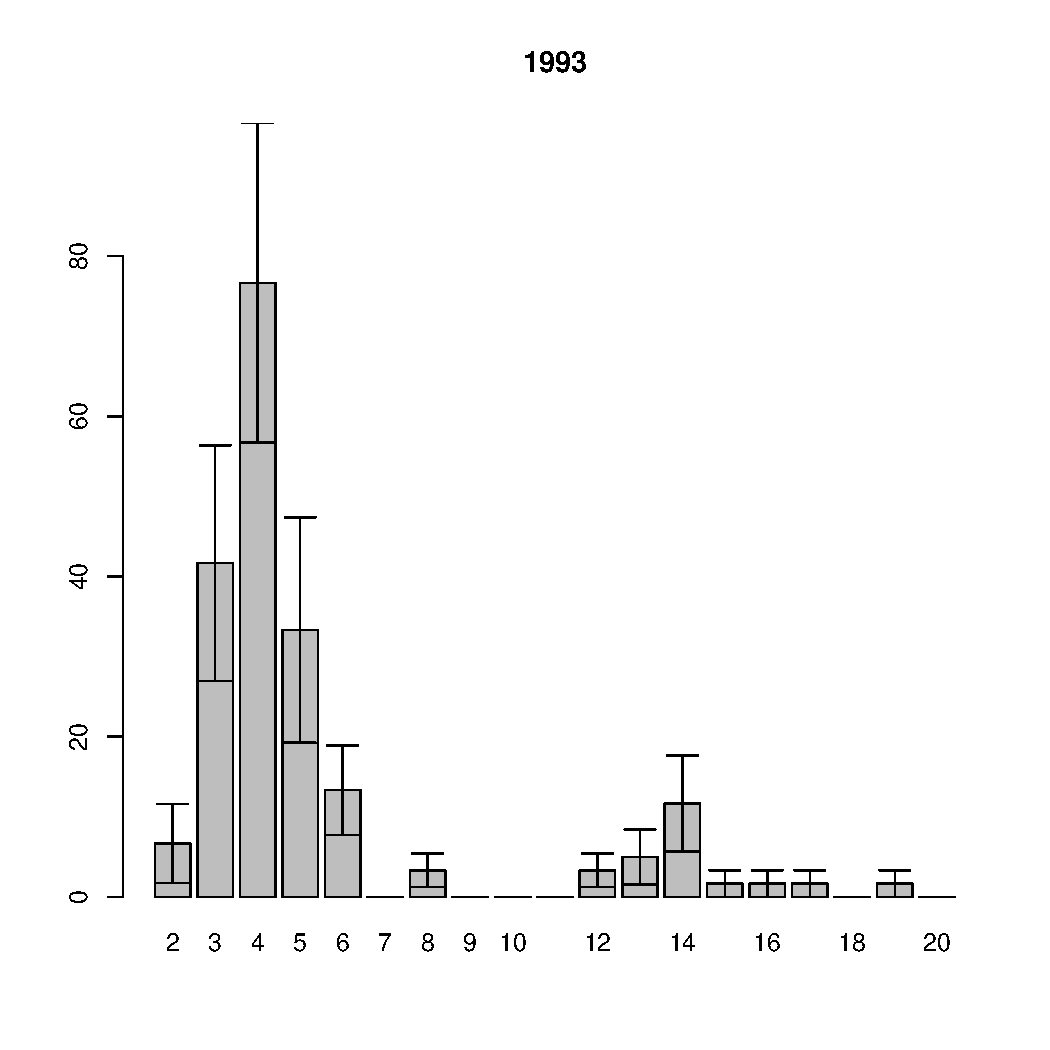
\includegraphics[width=65mm]{../White_Sea/Estuatiy_Luvenga/sizestr2_1993_.pdf}
\hfill
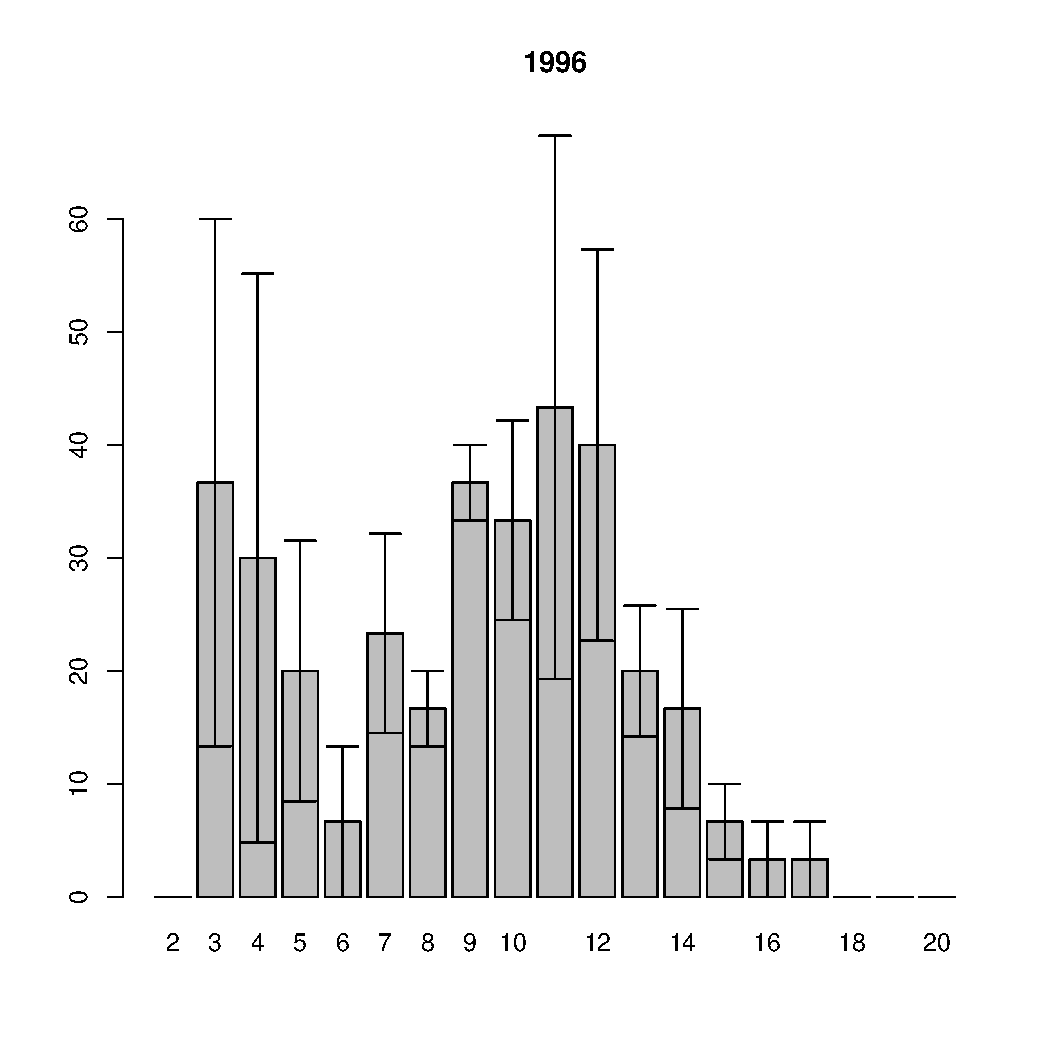
\includegraphics[width=65mm]{../White_Sea/Estuatiy_Luvenga/sizestr2_1996_.pdf}
\hfill
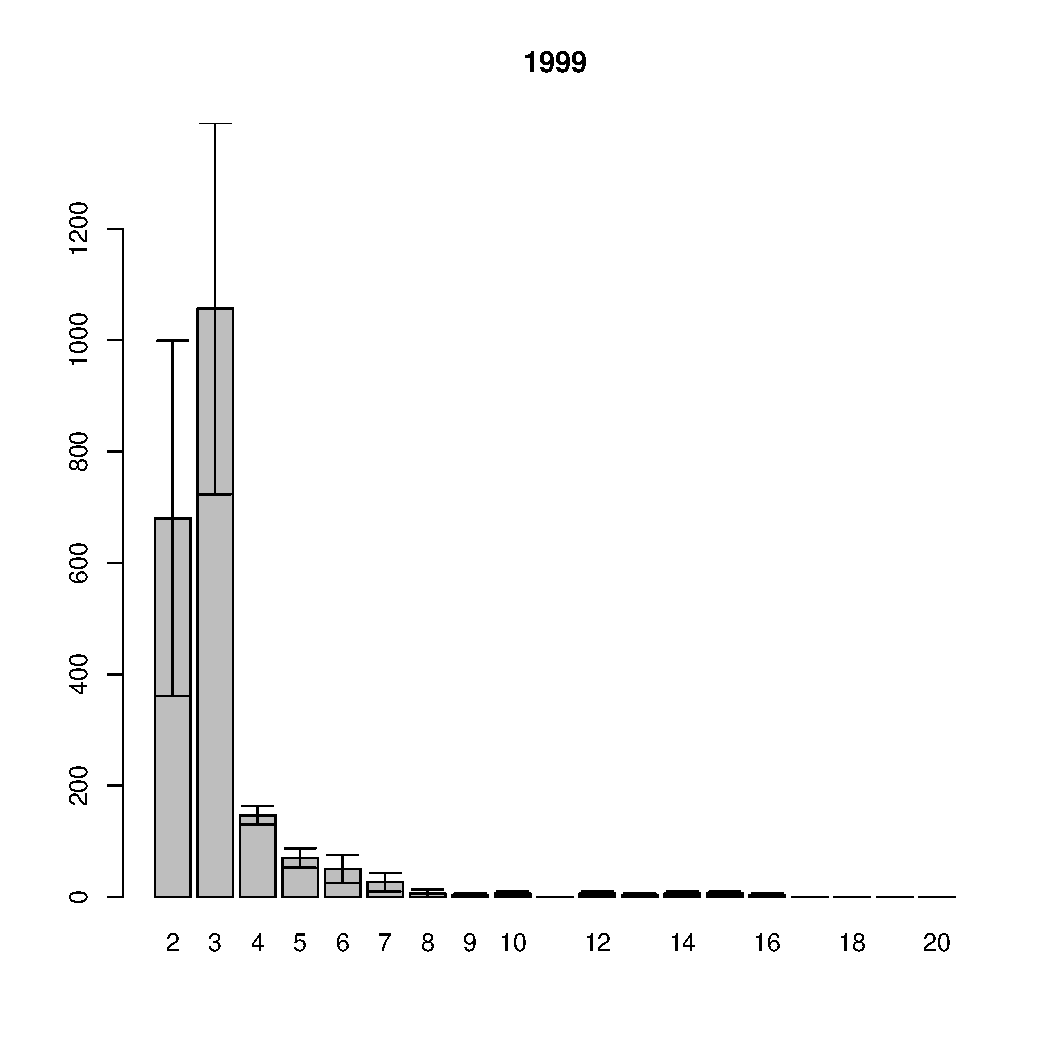
\includegraphics[width=65mm]{../White_Sea/Estuatiy_Luvenga/sizestr2_1999_.pdf}

\end{multicols}

%\smallskip

\begin{multicols}{3}
\hfill
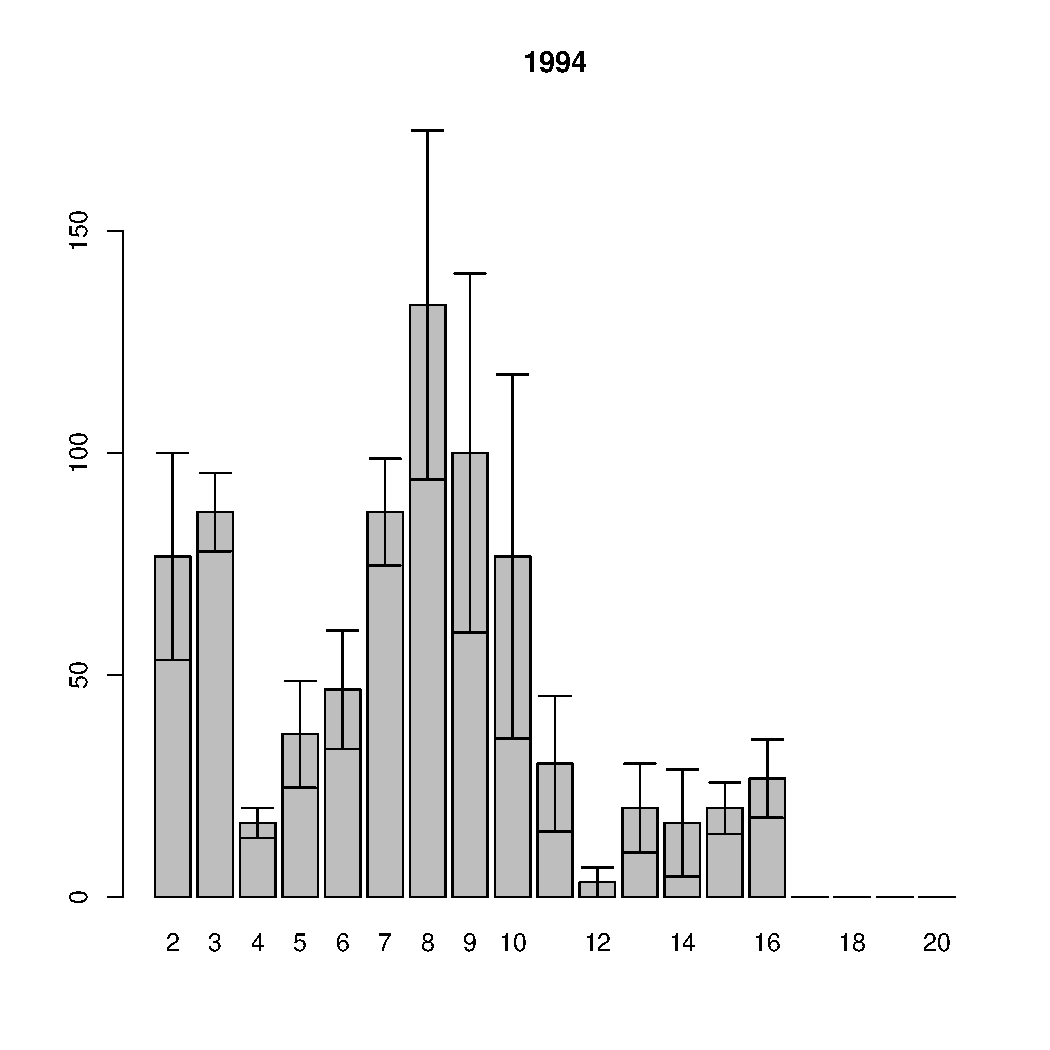
\includegraphics[width=65mm]{../White_Sea/Estuatiy_Luvenga/sizestr2_1994_.pdf}
\hfill
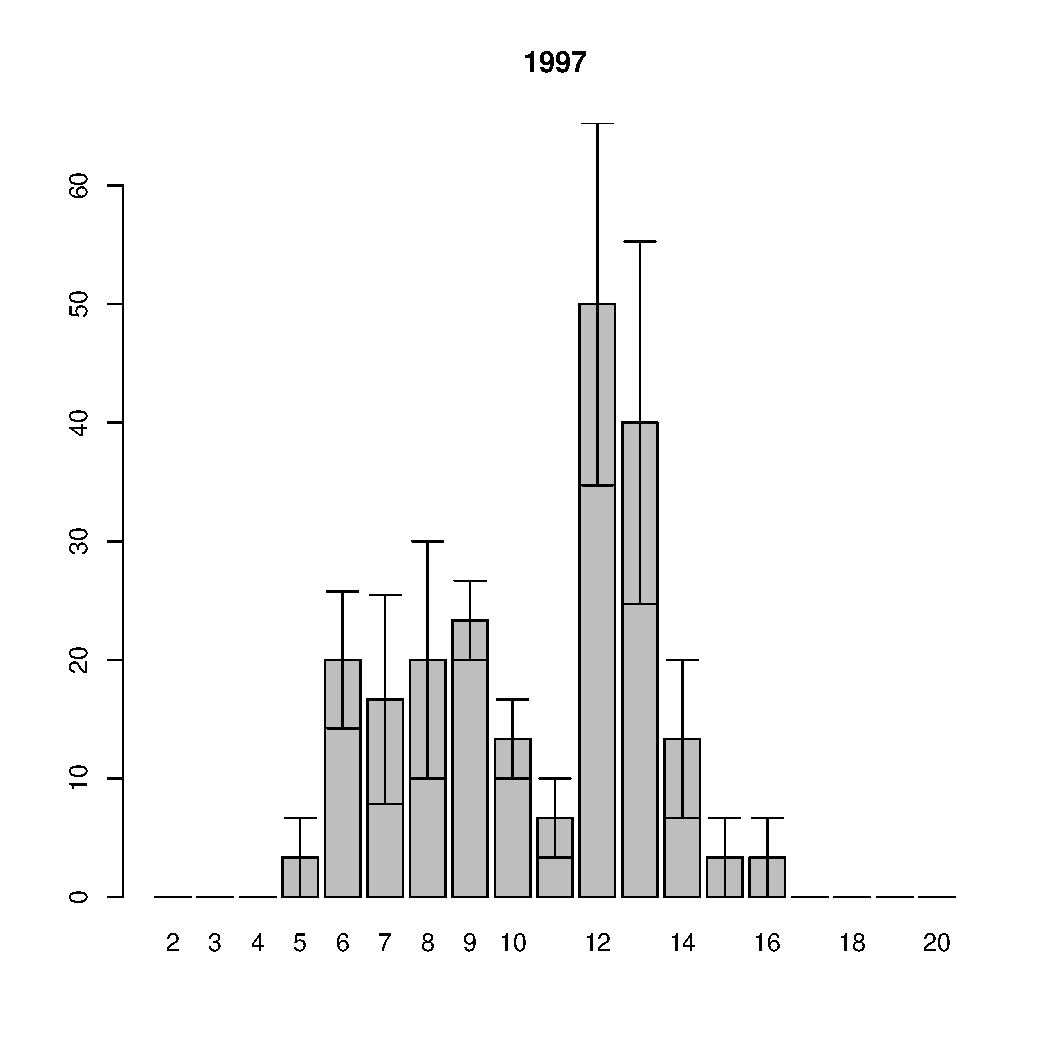
\includegraphics[width=65mm]{../White_Sea/Estuatiy_Luvenga/sizestr2_1997_.pdf}
\hfill
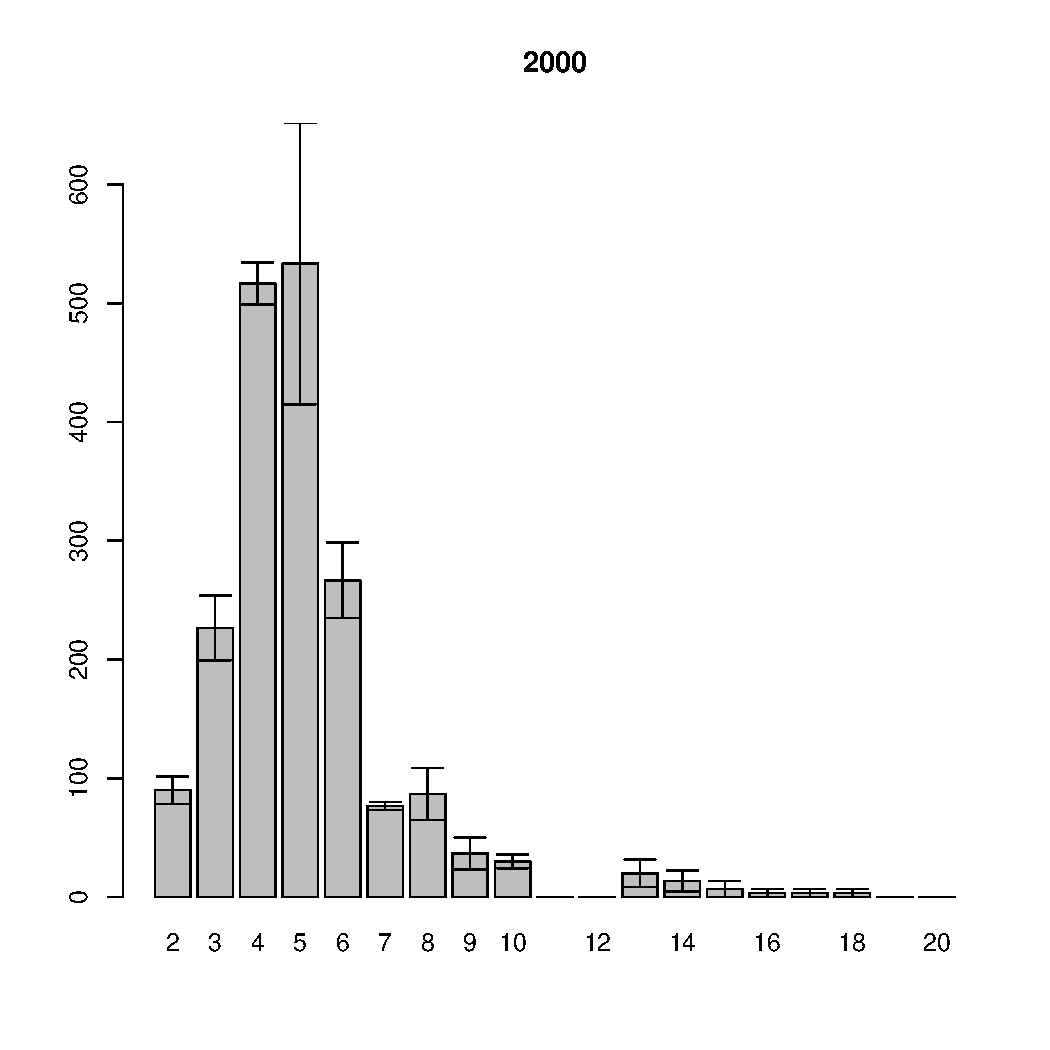
\includegraphics[width=65mm]{../White_Sea/Estuatiy_Luvenga/sizestr2_2000_.pdf}
\end{multicols}

%\smallskip


\caption{Размерная структура {\it Macoma balthica} в СГЛ эстуария р. Лувеньги}
\label{ris:size_str_estuary_Luv}
\end{figure}


\begin{figure}[h]

\begin{multicols}{3}
\hfill
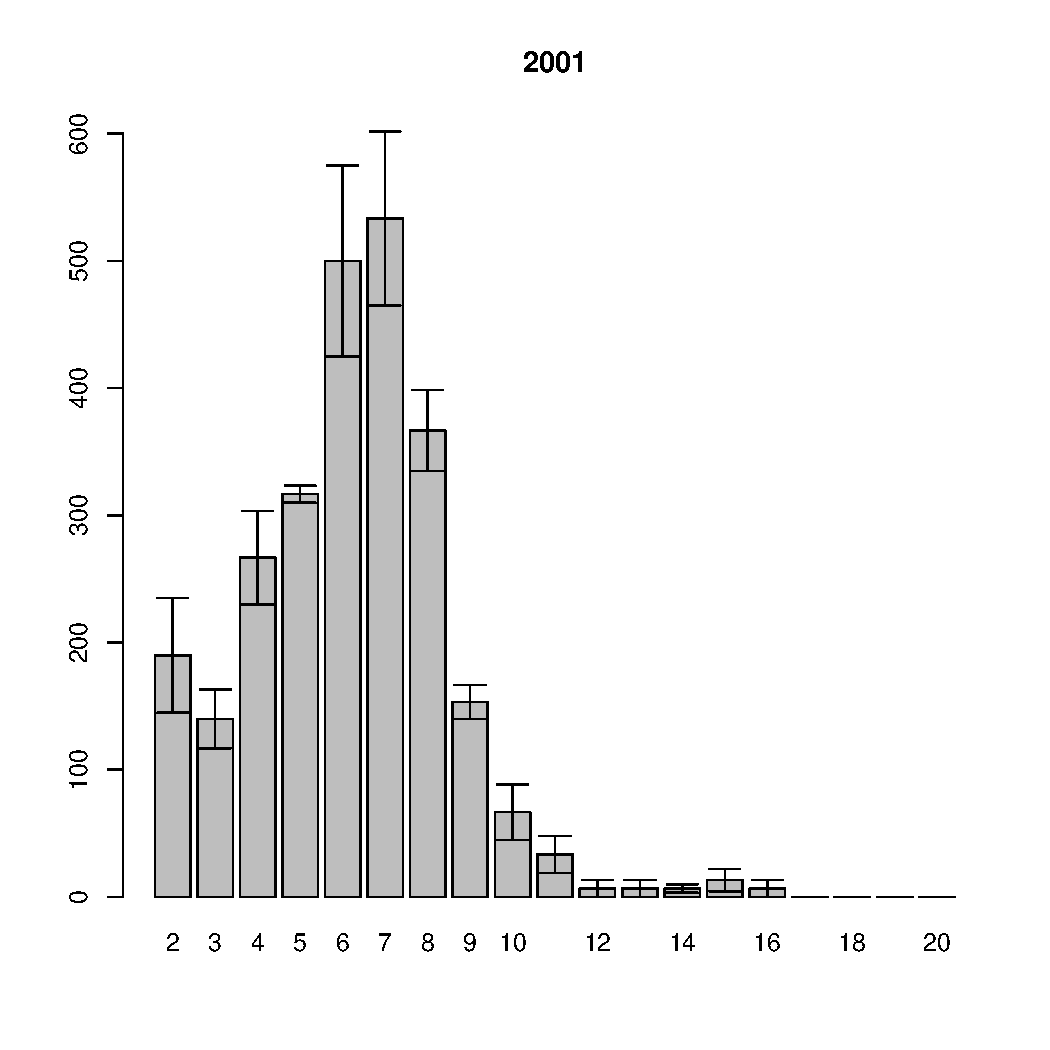
\includegraphics[width=65mm]{../White_Sea/Estuatiy_Luvenga/sizestr2_2001_.pdf}
\hfill
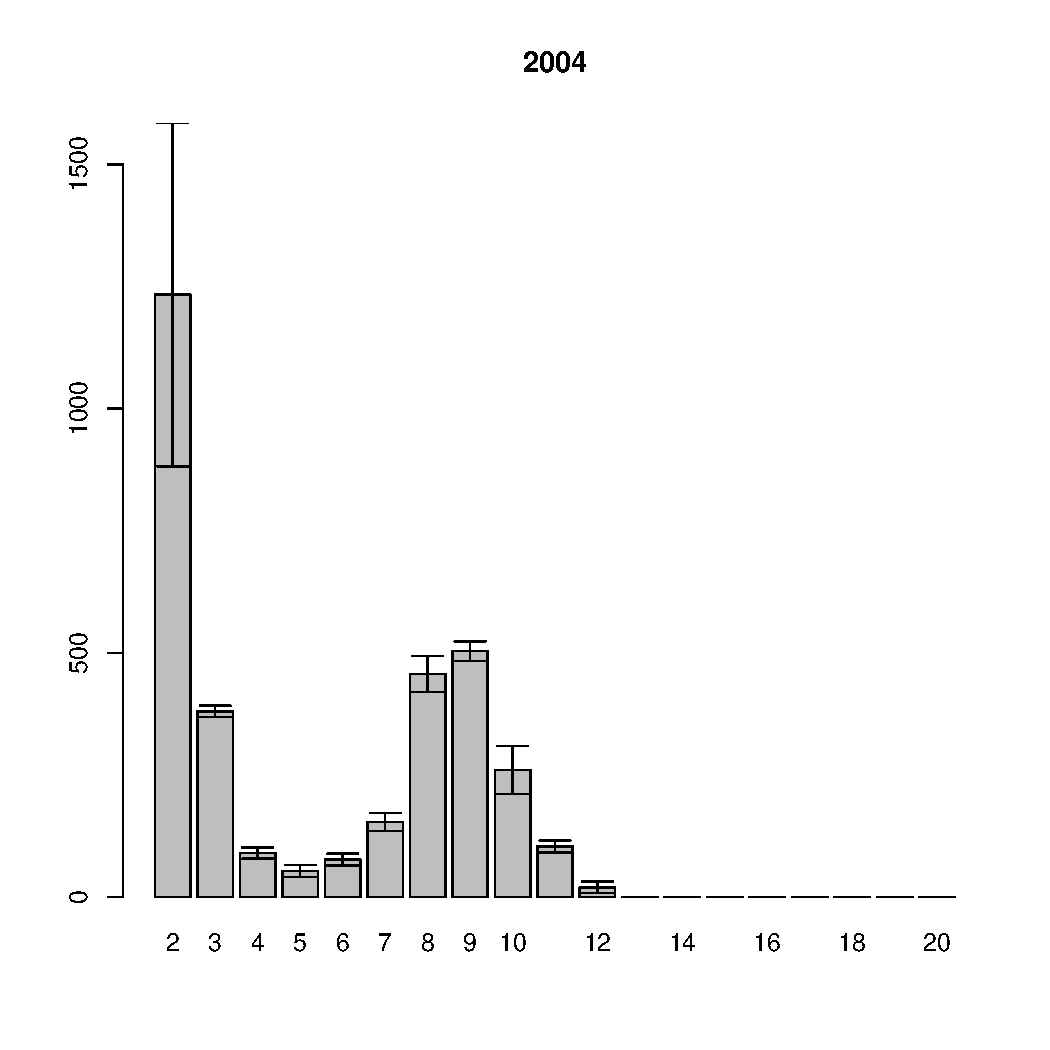
\includegraphics[width=65mm]{../White_Sea/Estuatiy_Luvenga/sizestr2_2004_.pdf}
\hfill
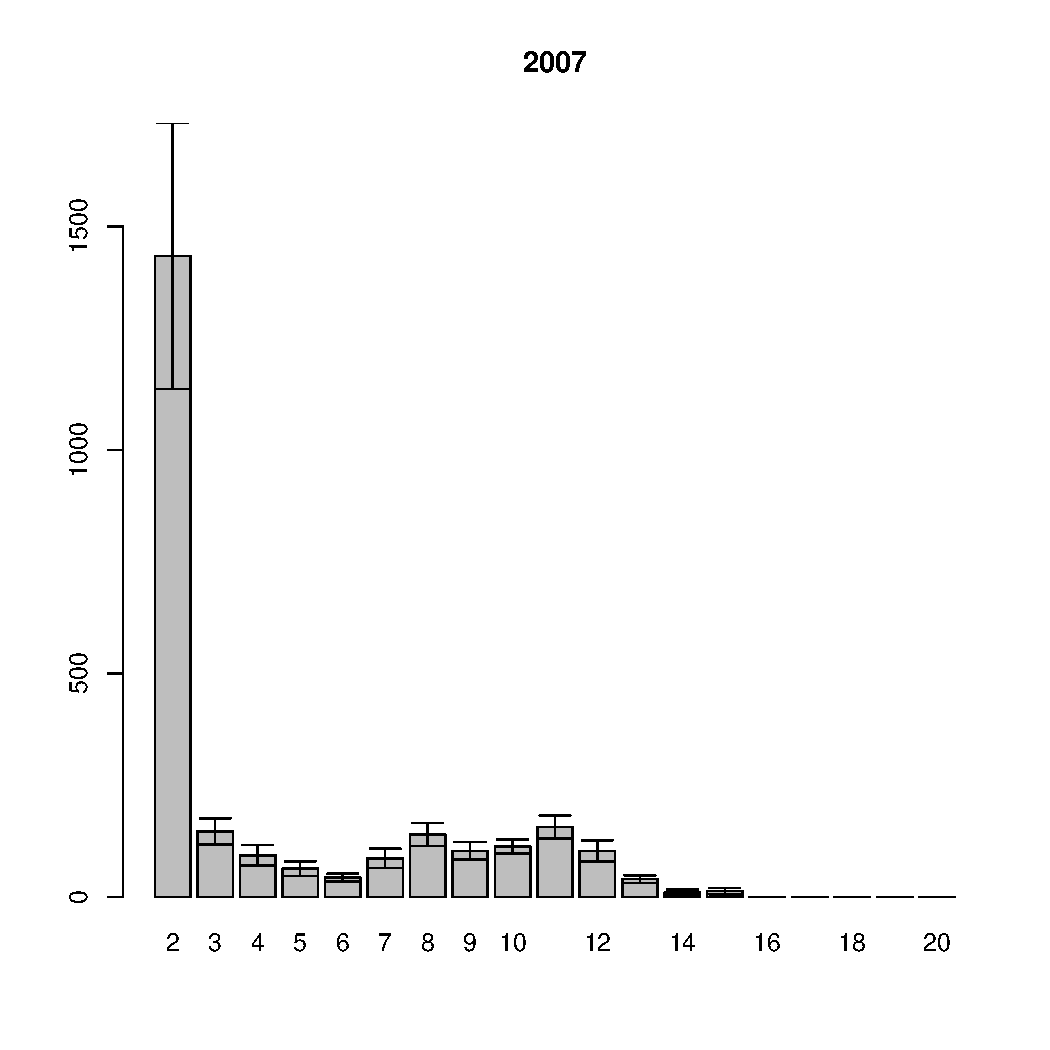
\includegraphics[width=65mm]{../White_Sea/Estuatiy_Luvenga/sizestr2_2007_.pdf}
\end{multicols}

\begin{multicols}{3}
\hfill
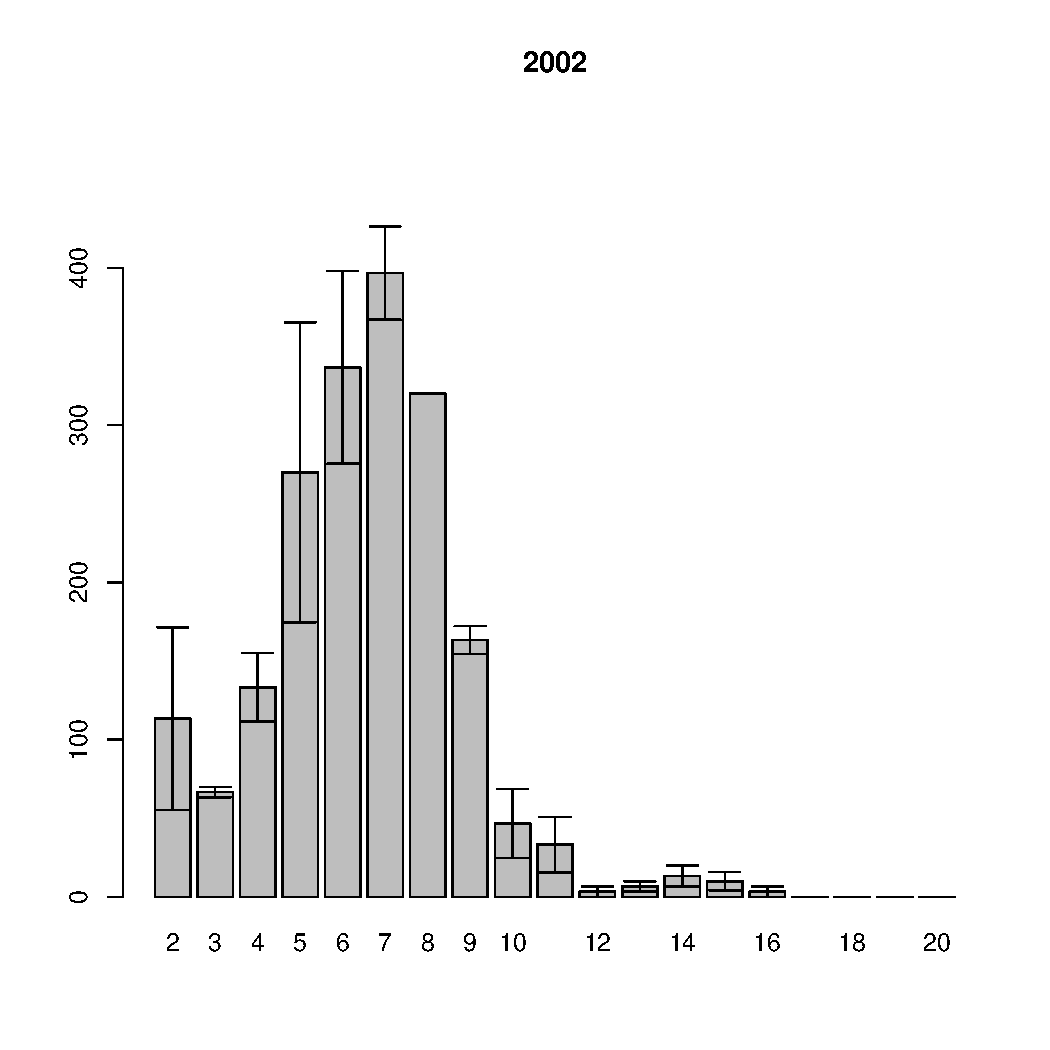
\includegraphics[width=65mm]{../White_Sea/Estuatiy_Luvenga/sizestr2_2002_.pdf}
\hfill
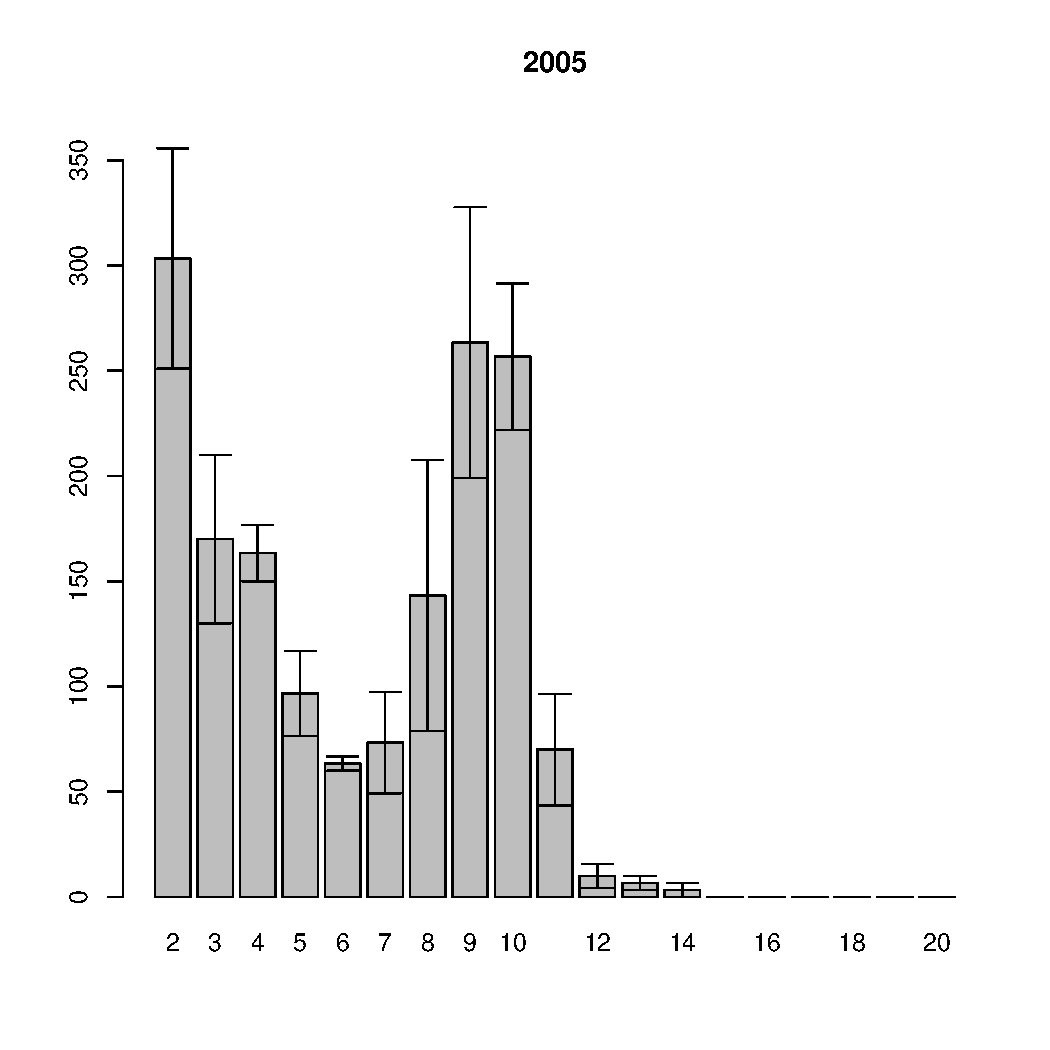
\includegraphics[width=65mm]{../White_Sea/Estuatiy_Luvenga/sizestr2_2005_.pdf}
\hfill
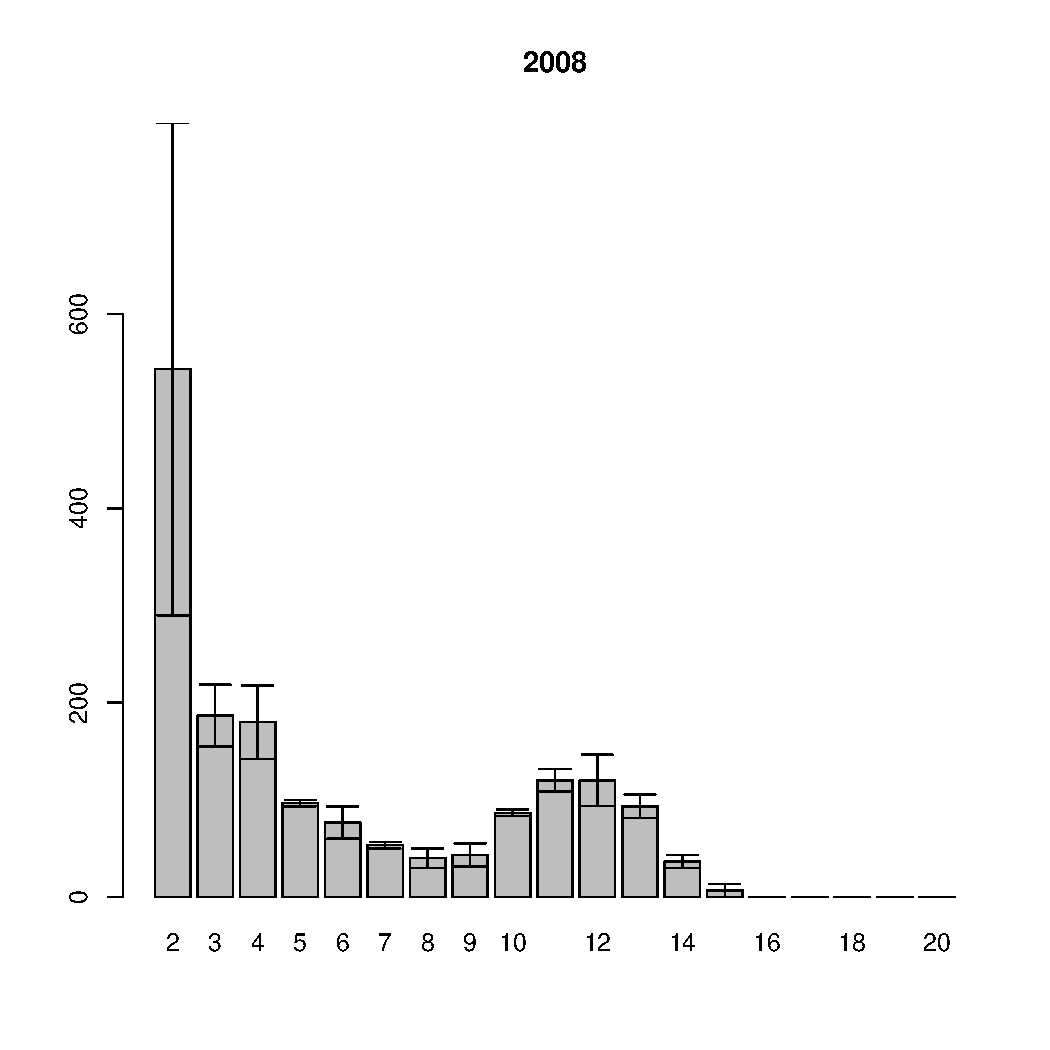
\includegraphics[width=65mm]{../White_Sea/Estuatiy_Luvenga/sizestr2_2008_.pdf}
\end{multicols}

%\smallskip


\begin{multicols}{3}
\hfill
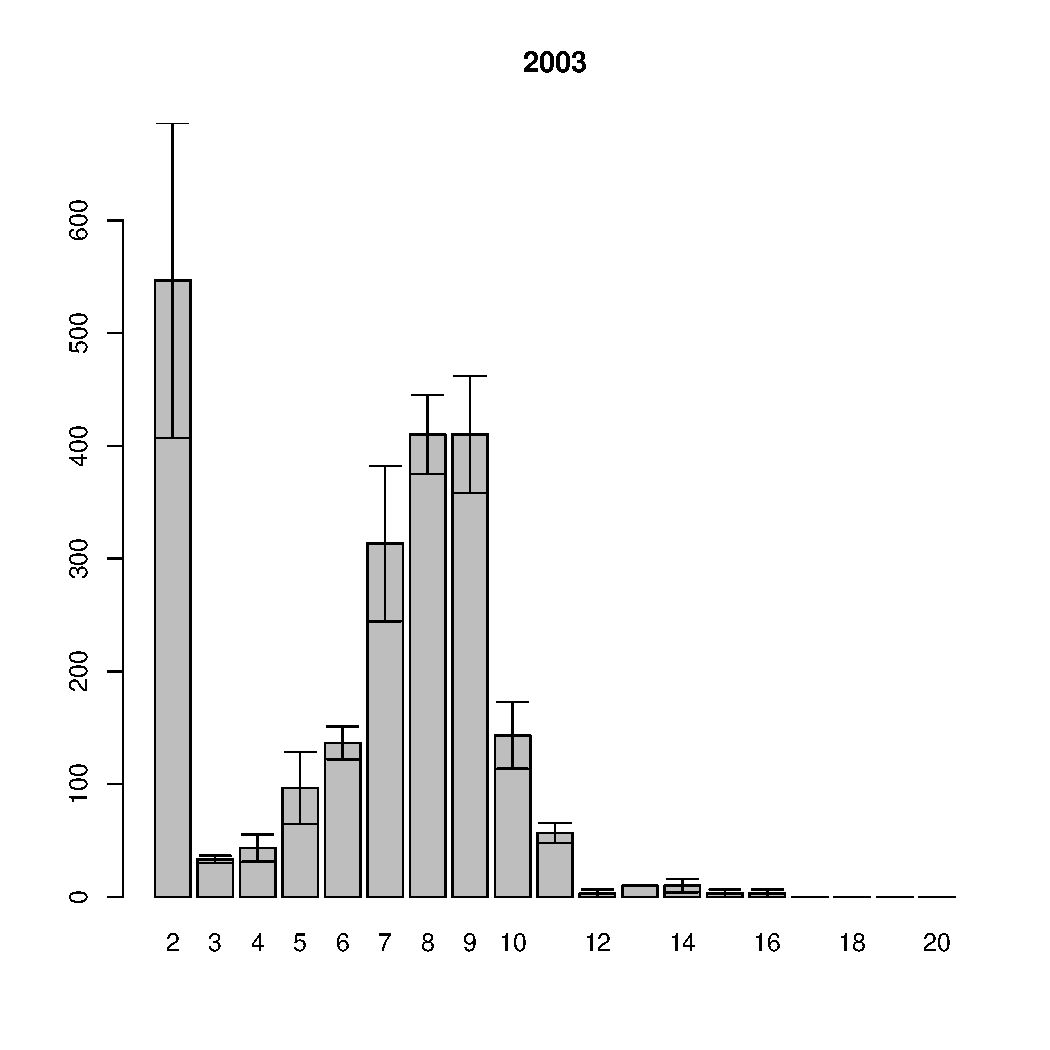
\includegraphics[width=65mm]{../White_Sea/Estuatiy_Luvenga/sizestr2_2003_.pdf}
\hfill
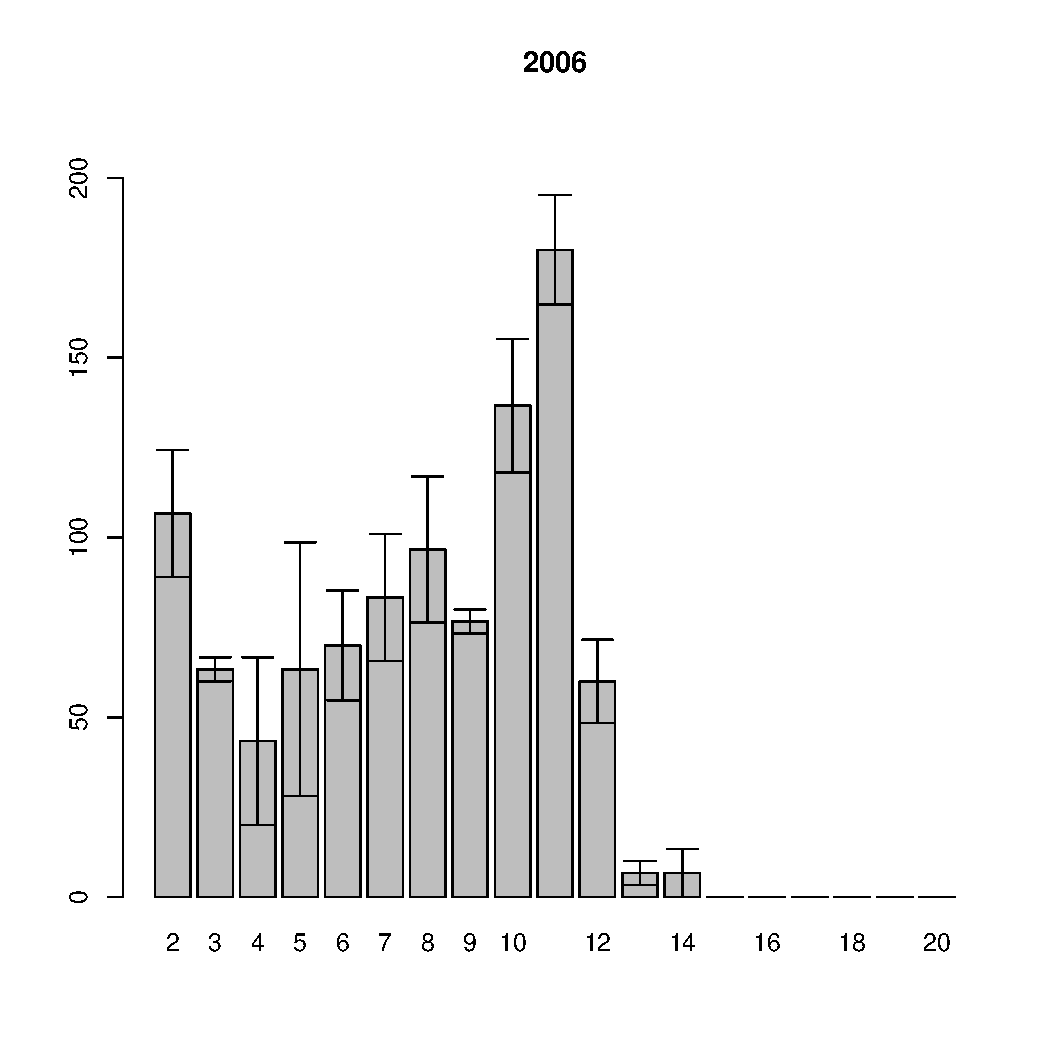
\includegraphics[width=65mm]{../White_Sea/Estuatiy_Luvenga/sizestr2_2006_.pdf}
\hfill
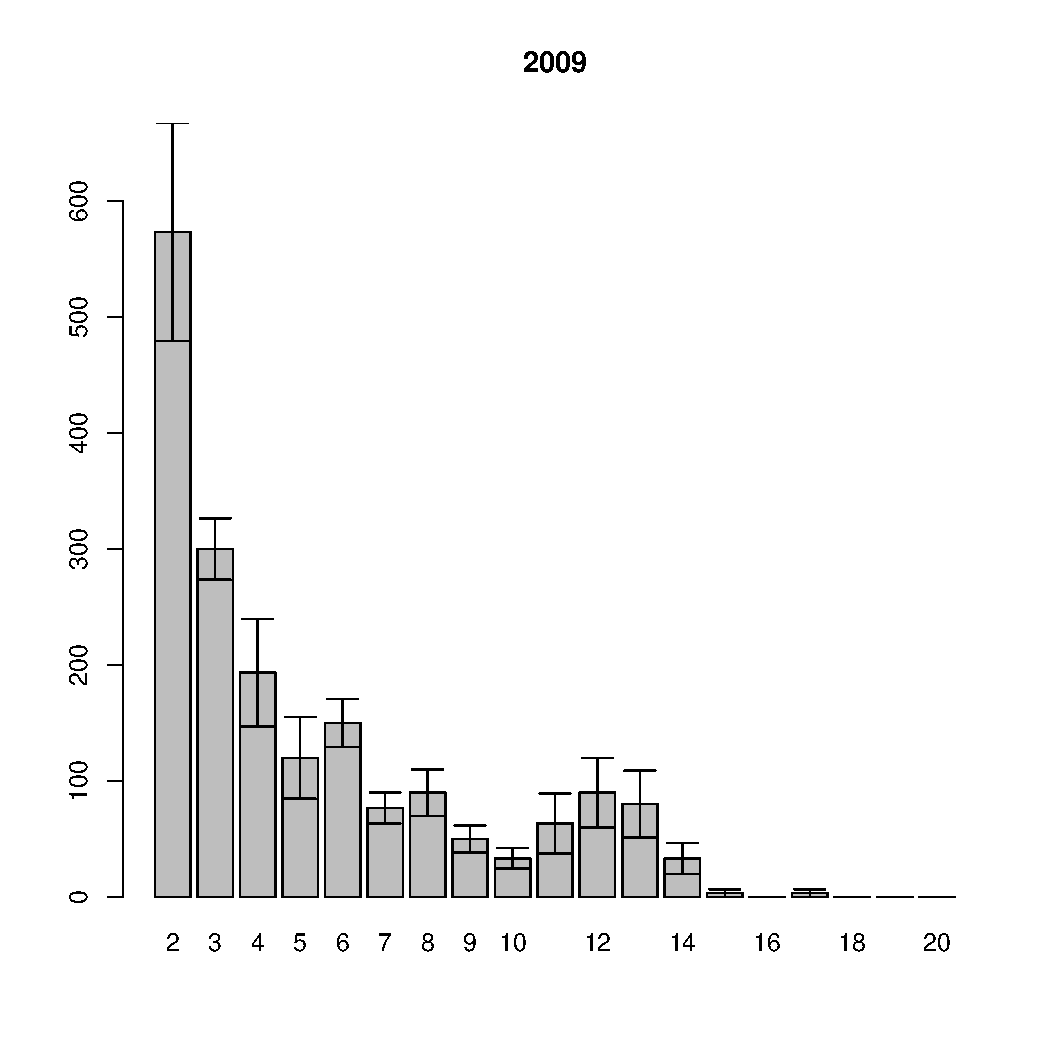
\includegraphics[width=65mm]{../White_Sea/Estuatiy_Luvenga/sizestr2_2009_.pdf}
\end{multicols}

%\smallskip


%\caption{Размерная структура {\it Macoma balthica} в СГЛ эстуария р. Лувеньги}
%\label{ris:size_str_estuaty_Luv}
\begin{center}
Рис. \ref{ris:size_str_estuary_Luv} (продолжение). Размерная структура {\it Macoma balthica} в СГЛ эстуария р. Лувеньги

\end{center}
\end{figure}


\begin{figure}[h]

\begin{multicols}{3}
\hfill
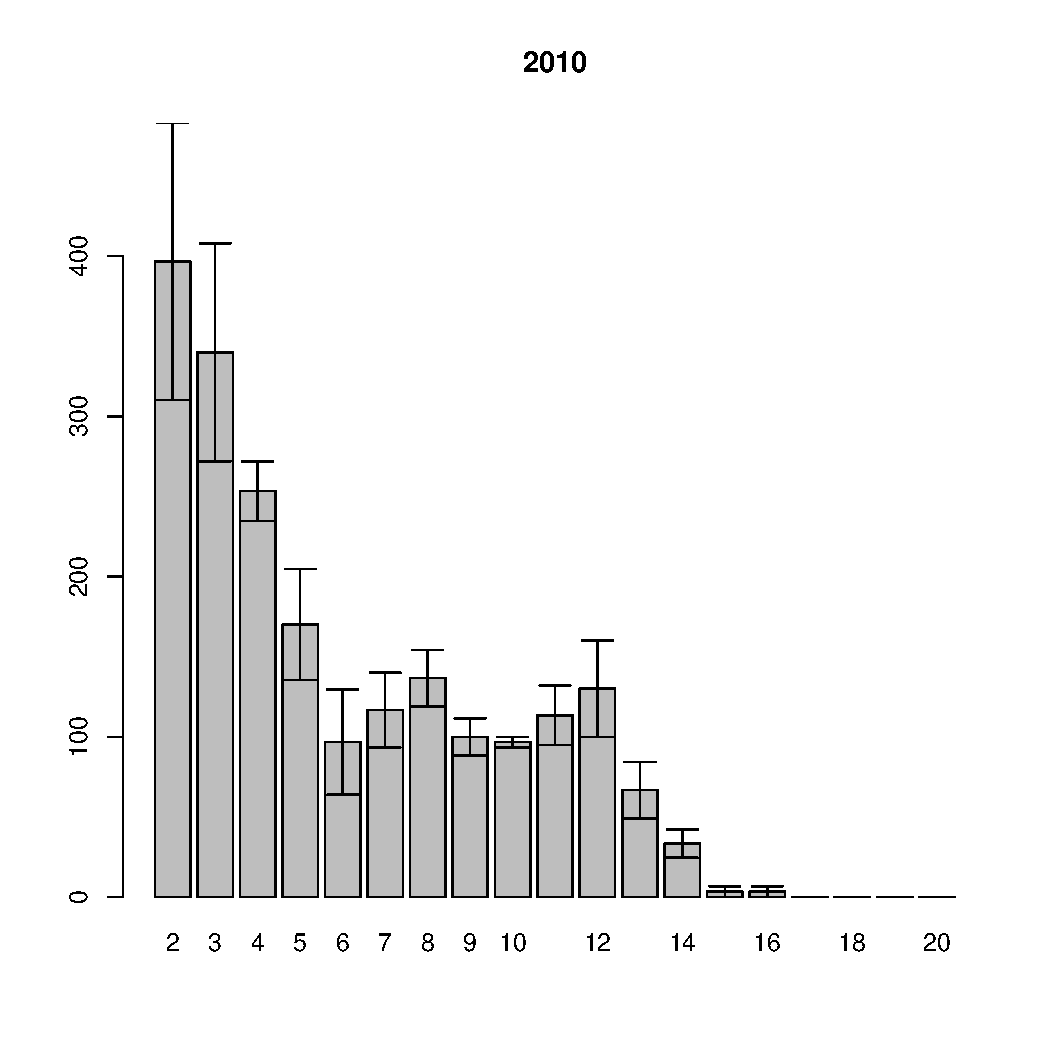
\includegraphics[width=65mm]{../White_Sea/Estuatiy_Luvenga/sizestr2_2010_.pdf}
\hfill
%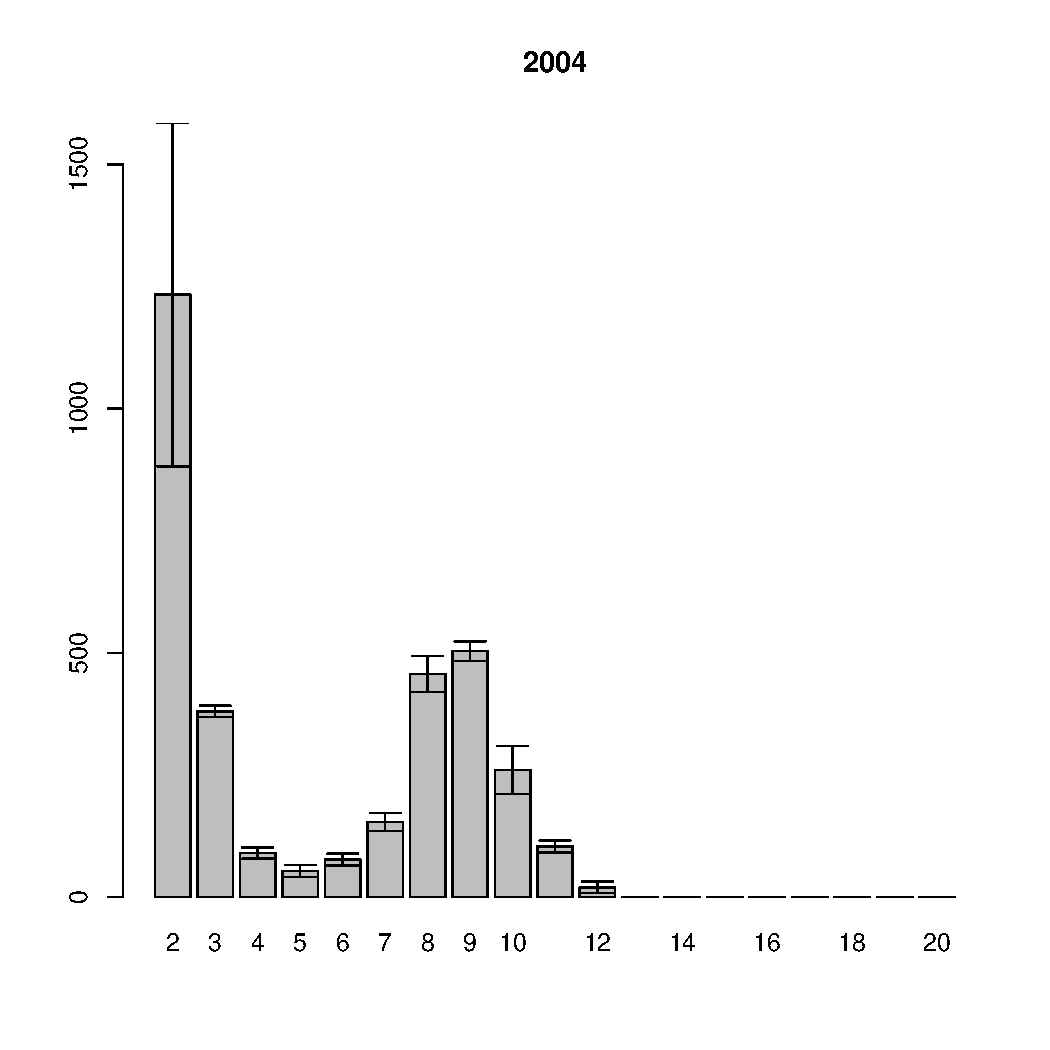
\includegraphics[width=65mm]{../White_Sea/Estuatiy_Luvenga/sizestr2_2004_.pdf}
%\hfill
%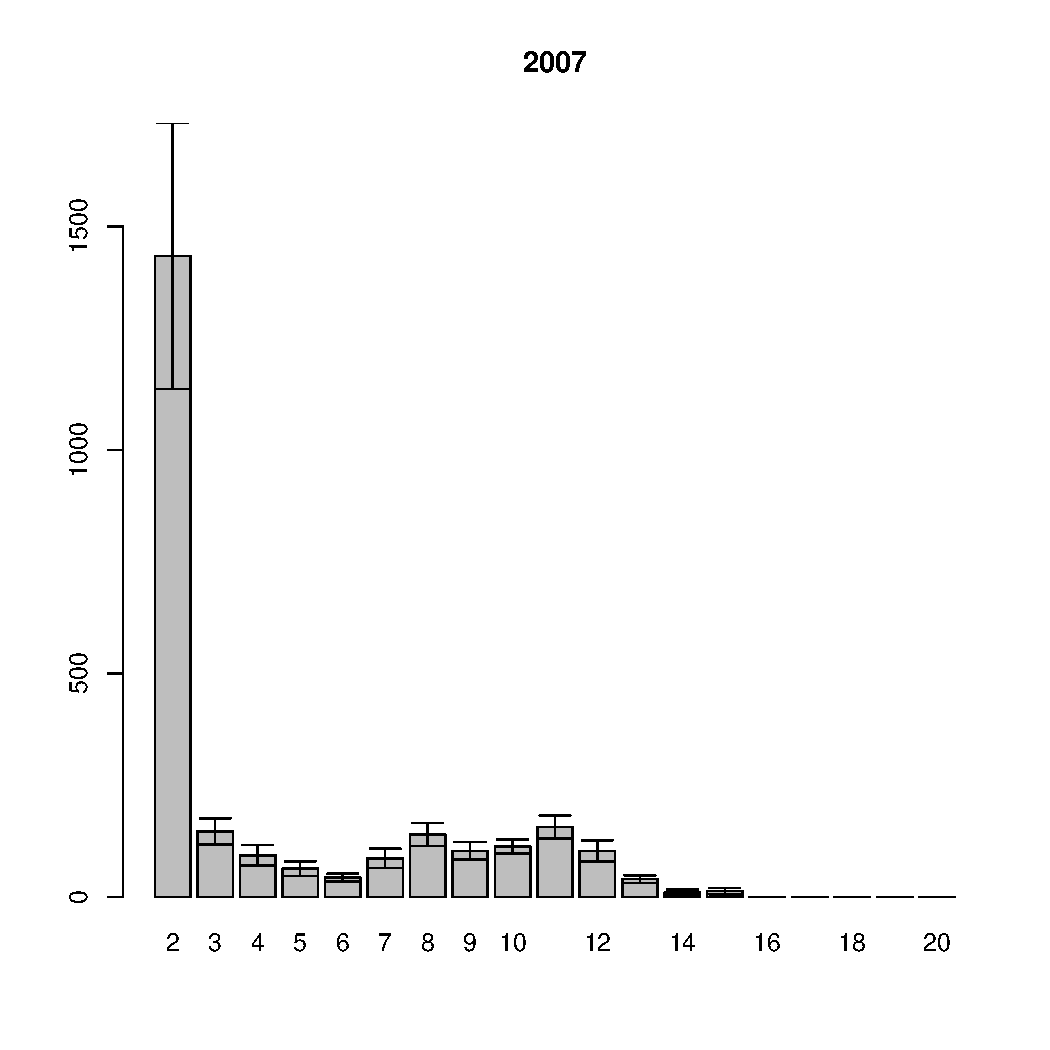
\includegraphics[width=65mm]{../White_Sea/Estuatiy_Luvenga/sizestr2_2007_.pdf}
\end{multicols}

\begin{multicols}{3}
\hfill
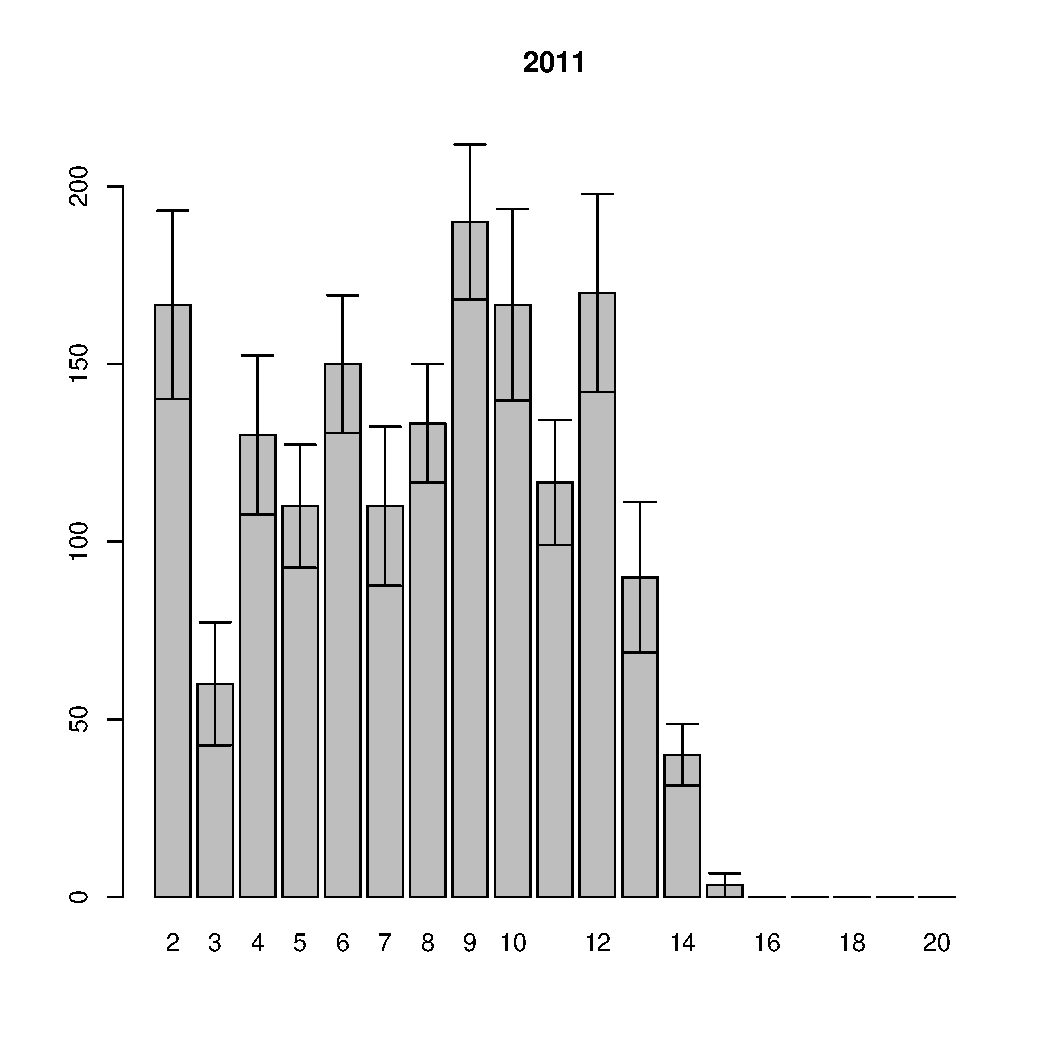
\includegraphics[width=65mm]{../White_Sea/Estuatiy_Luvenga/sizestr2_2011_.pdf}
%\hfill
%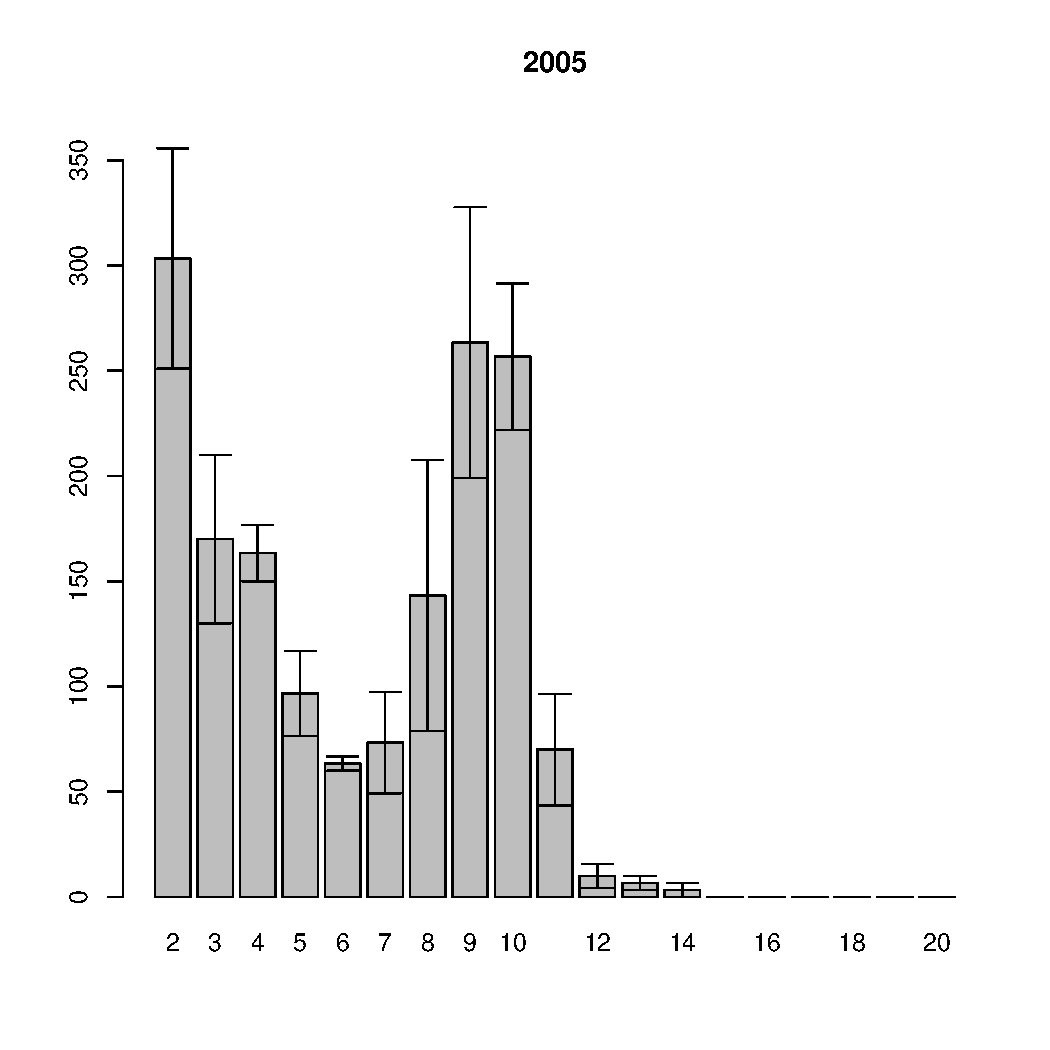
\includegraphics[width=65mm]{../White_Sea/Estuatiy_Luvenga/sizestr2_2005_.pdf}
%\hfill
%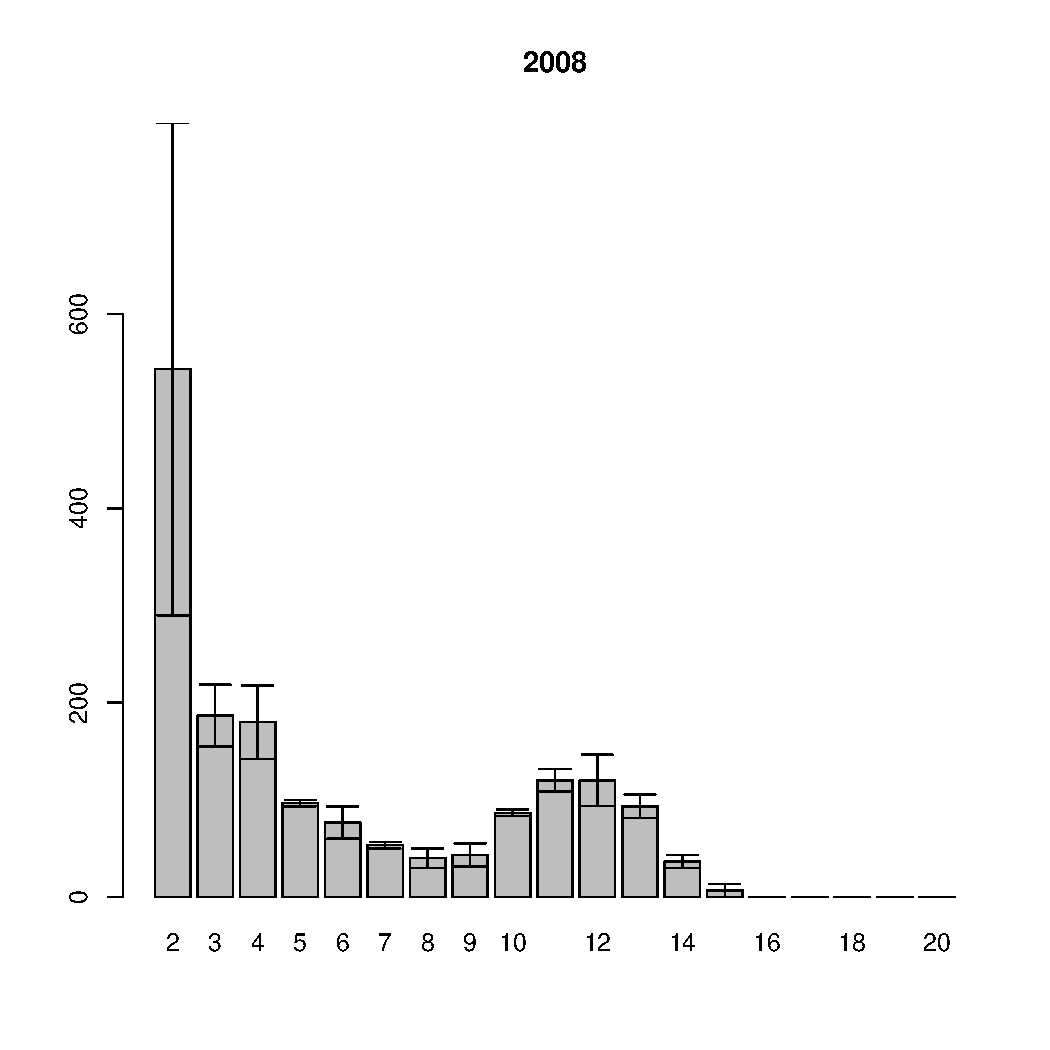
\includegraphics[width=65mm]{../White_Sea/Estuatiy_Luvenga/sizestr2_2008_.pdf}
\end{multicols}

%\smallskip


\begin{multicols}{3}
\hfill
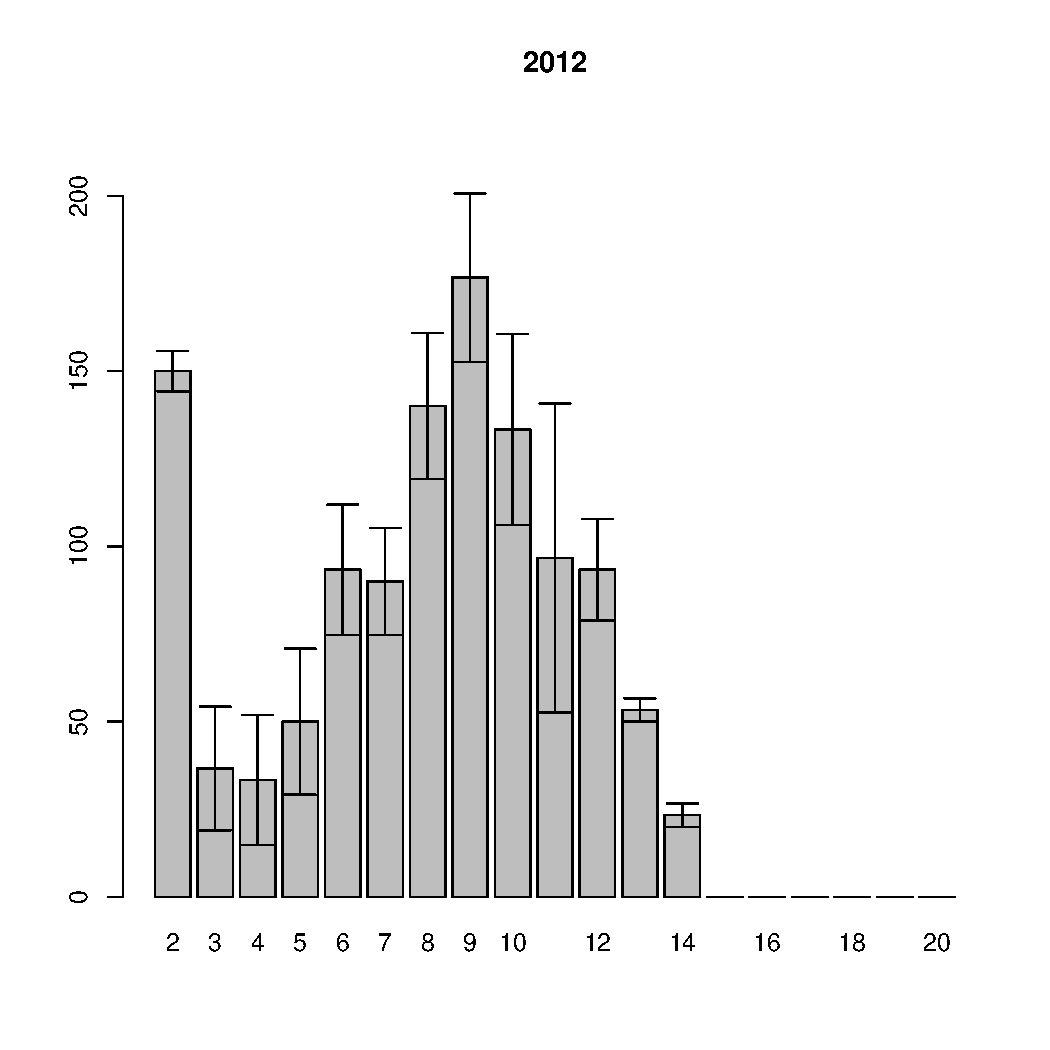
\includegraphics[width=65mm]{../White_Sea/Estuatiy_Luvenga/sizestr2_2012_.pdf}
%\hfill
%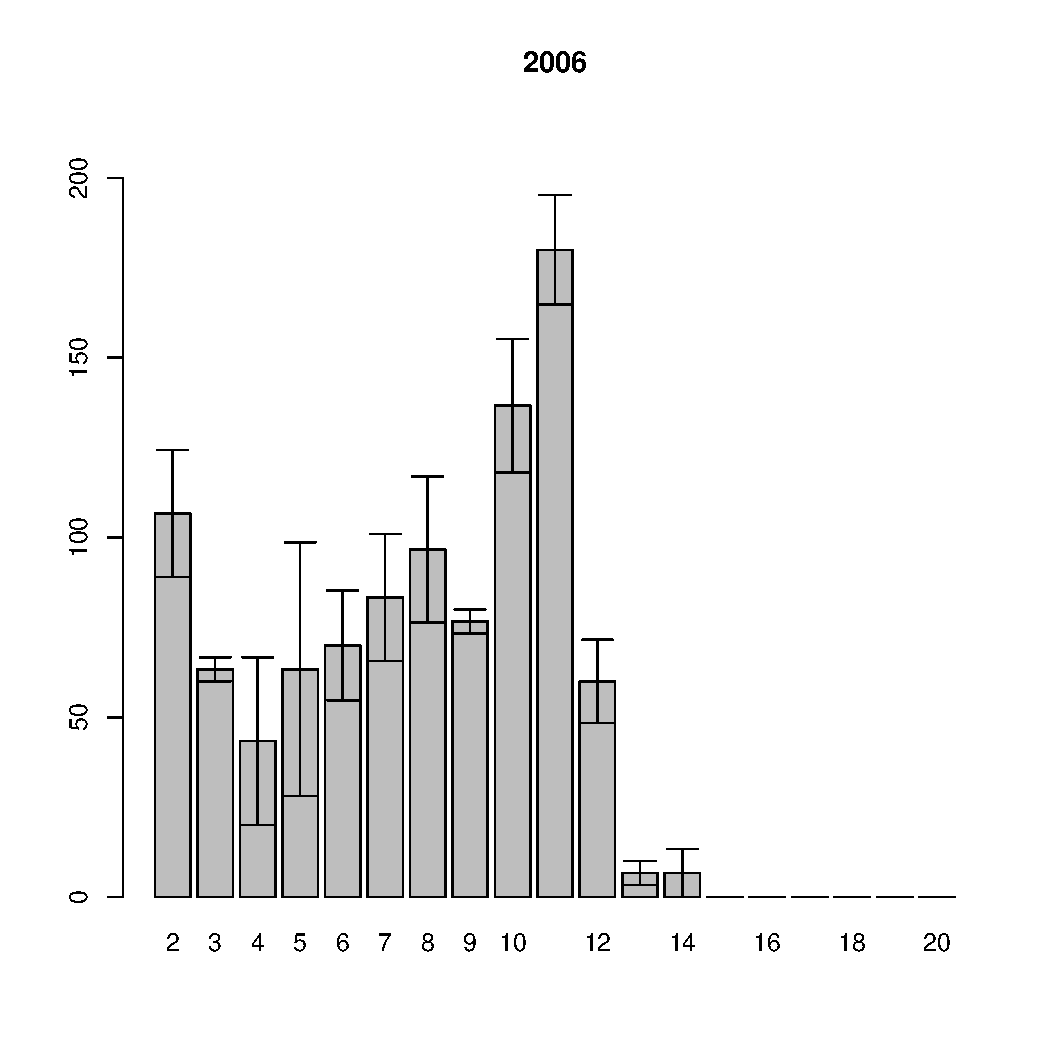
\includegraphics[width=65mm]{../White_Sea/Estuatiy_Luvenga/sizestr2_2006_.pdf}
%\hfill
%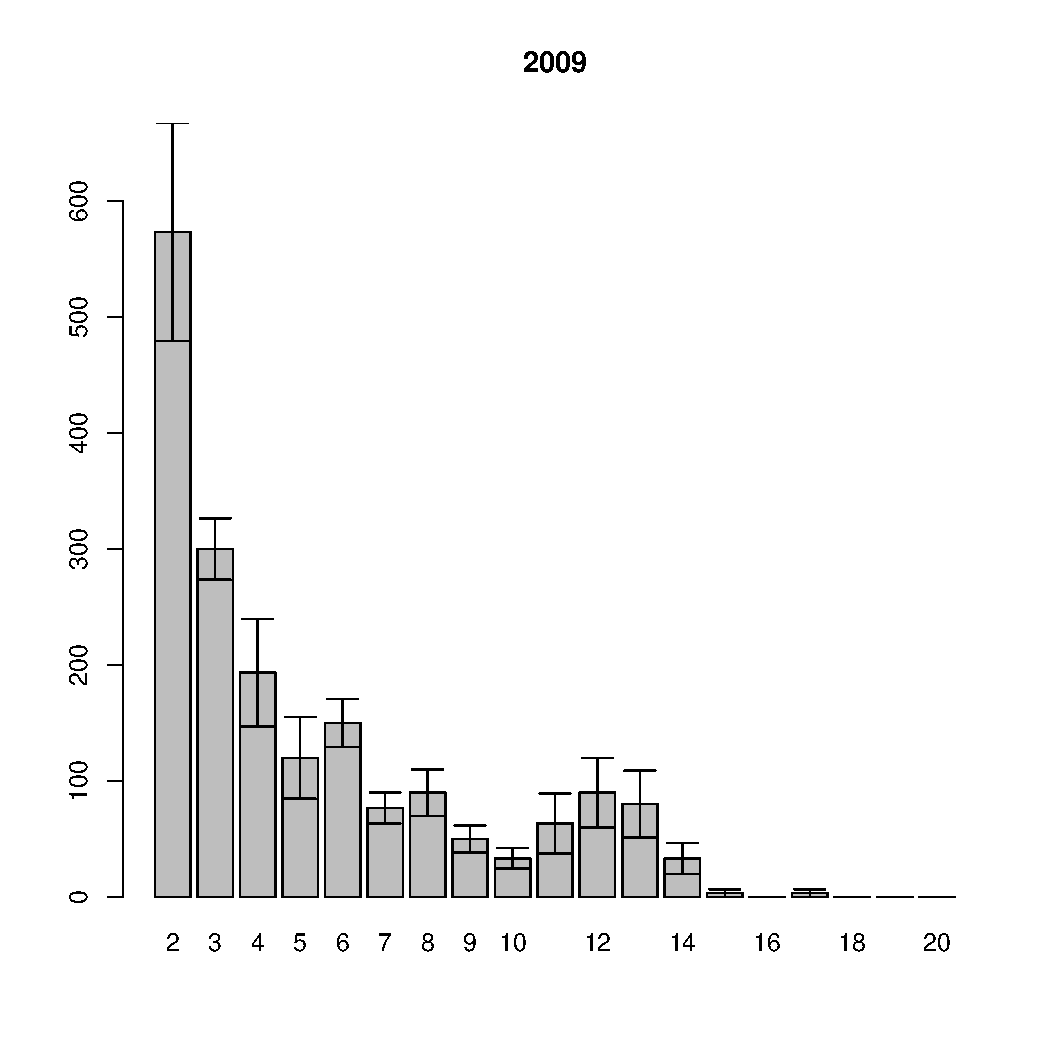
\includegraphics[width=65mm]{../White_Sea/Estuatiy_Luvenga/sizestr2_2009_.pdf}
\end{multicols}

%\smallskip


%\caption{Размерная структура {\it Macoma balthica} в СГЛ эстуария р. Лувеньги}
%\label{ris:size_str_estuaty_Luv}
\begin{center}
Рис. \ref{ris:size_str_estuary_Luv} (продолжение). Размерная структура {\it Macoma balthica} в СГЛ эстуария р. Лувеньги

\end{center}
\end{figure}

\end{document}
